%%
%% This is file `mcmthesis-demo.tex',
%% generated with the docstrip utility.
%%
%% The original source files were:
%%
%% mcmthesis.dtx  (with options: `demo')
%%
%% -----------------------------------
%%
%% This is a generated file.
%%
%% Copyright (C)
%%     2010 -- 2015 by Zhaoli Wang
%%     2014 -- 2016 by Liam Huang
%%     2016 -- 2018 by Xuehan Sun
%%
%% This work may be distributed and/or modified under the
%% conditions of the LaTeX Project Public License, either version 1.3
%% of this license or (at your option) any later version.
%%
%% This work has the LPPL maintenance status `maintained'.
%%
%% The Current Maintainer of this work is Xuehan Sun.
%%
\documentclass{mcmthesis}
\mcmsetup{CTeX = false,   % 使用 CTeX 套装时,设置为 true
        tcn = 011, problem = B,
        sheet = true, titleinsheet = true, keywordsinsheet = true,
        titlepage = true}
\usepackage{palatino}
\usepackage{mwe}
\usepackage{graphicx}
\usepackage{subcaption}
\usepackage{float}
\usepackage{multirow}
\usepackage{indentfirst}
\usepackage{gensymb}
\usepackage[ruled,lined,commentsnumbered]{algorithm2e}
\usepackage{geometry}
\usepackage{subfigure}
\geometry{left=2cm,right=2cm,top=2cm,bottom=2cm} %%页边距

\begin{document}
\linespread{0.6} %%行间距
\setlength{\parskip}{0.5\baselineskip} %%段间距
\title{Bus Booking Platform: A guarantee for quick leaving}

\date{\today}
	\begin{abstract}
	
		\begin{keywords}
		
		\end{keywords}
	\end{abstract}

\maketitle

\tableofcontents

\newpage

\section{Introduction}
\subsection{Restatement of the Problem}
Shanghai Pudong International Airport is one of two international airports of Shanghai and a major aviation hub of China. Pudong Airport mainly serves international flights.

\begin{figure}[h]
    \centering
    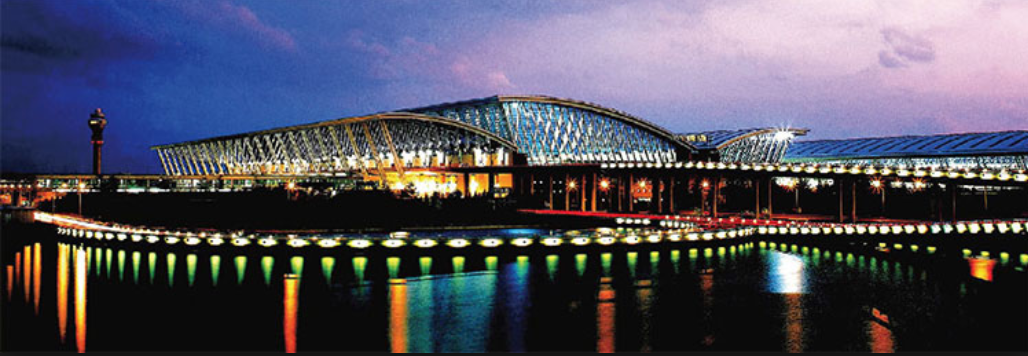
\includegraphics[width=0.8\textwidth]{SPIA.png}
    \caption{Shanghai Pudong International Airport \cite{Google_SPIA}}
    \label{fig:SPIA}
\end{figure}

As a huge rendezvous for many passengers, Pudong Airport has put forward a large number of measures to evacuate passengers. This operates quite well during daytime. However, during midnight period(23:00-02:00) when travellers get off from the red-eye flight, there is not enough transport capabilities to ensure passengers arrive home in a short time. According to official statistics from Shanghai Traffic Management Bureau(STMB), around 10,000 passengers are stranded at the airport, waiting for a home-ride for a long duration.

Therefore, a new service APP \emph{bus-booking platform} is introduced by STMB to promote a higher-quality service. \emph{The bus-booking platform} dispatch orders and carefully pre-planned routes to each bus, relying on real-time demands from passengers. This leads to a shorter and cheaper commuting time, combining existing benefits of bus service and car-hailing.

\subsection{Our Work}







\section{Assumptions}

Our model makes four assumptions as follows:

\begin{enumerate}
	\item In the phase of modeling, we consider each passenger as the same individual subject, and the taxi and bus GPS data on January 31st, 2007 statistically representative. We assume each passenger has the same standard for user satisfaction, namely satisfied if bus is available while unsatisfied if not. Besides, we suppose there's little difference between the GPS data on the date we choose and others'.
	\item The GPS data typically reflects passengers' demands for buses' destinations. Since it's at deep night, there's few traffic jams. Besides, waiting time at the crossroads are randomly equal. 
	\item There is only one starting station, namely the Airport Station, and 50 terminal stations to choose from. All passengers need to go to this station to enjoy our bus-booking service. We don't take different airline landing site into account. 
	\item All the buses are the same, and seat 33 people. We simplify the bus to be used as the same standard bus, which has a fixed seat of 33 passengers averagely, based on our online research and calculation. Additionally, traffic accidents are ignored because it is rare, especially at night.
\end{enumerate}

\section{Nomenclature}
In this paper, we use the nomenclature in Table\ref{tab:Nomen} to describe our model. Other symbols that are used only once will be described later in the context.
\begin{table}
    \centering
    \caption{Nomenclature}
    \label{tab:Nomen}
    \begin{tabular}{c c}
\hline
    	Symbol & Definition\\
\hline
	$x$ & The longitude of each map point\\
	$y$ & The latitude of each map point\\
	$P(x,y)$ & The population density of each map point\\
	$T(x,y)$ & The taxi and bus GPS-recognized position density $i$\\
	$M(x,y)$ & The combined probability distribution of each map point\\
	$P_f$ & Acceptable risk ratio\\
	$Q(X_i;t)$ & Volumetric flow rate at time $t$ for dam $i$\\
\hline
    \end{tabular}
\end{table}





\section{Statement of our model}
In this section, we will discuss all detailed symbols about our model. This model

\subsection{Destination Selection Model}
In our model, we need to select 50 hot destinations for passengers to choose from as their destination station. $P(x,y)$ is generated through an officially given chart. We use the legend given and color distribution, as well as noise reduction methods to get the two-dimension mathematical function. $T(x,y)$ is acquired through the given dataset. Form the given dataset, we assign a limited value to each existing map point. We take the longitude, latitude, speed, and status(occupied) into account, after which we apply convolution techniques to relevant values in order to form a two-dimension mathematical function.

\begin{figure}[htbp]
\centering    %居中
 


We use the product of two functions as our final selection function to estimate potential destinations.

\begin{equation}\label{1steq}
    M(x,y) = P(x,y) \times T(x,y)
\end{equation}

The larger the product of the two functions for each map point, the greater possibility for it to be chosen as a destination. With this formula, we generate a chart on which we can preliminarily see the distribution of potential sites.

\subsection{Route Selection Model}
\subsection{Bus Dispatching Model}




\begin{figure}[htbp]
    \centering
    \includegraphics[height=7cm,width=8cm]{figures/pd.jpg}
    \caption{The population density of Shanghai in 2013~\cite{dqxxkx_ppl}}
    \label{fig:population density}
\end{figure}






\section{Model Analysis}
\subsection{Sensitivity Analysis}
\subsection{Strengths and Weaknesses}
\subsubsection{Strengths}
\subsubsection{Weaknesses}

\section{Conclusion}

\newpage
\section{Advertisement}
Bushub is a novel bus booking platform app. We aim to offer each passenger off the plane a quick arrival at the destination. \\
Advantages:

\begin{figure}[htbp]
    \centering
    
\includegraphics[height=6cm,width=10cm]{figures/Bushublogo.png}
\end{figure}

\subsection{Usage}
\begin{itemize}
\item Destinations:
\item Price \& Time Intervals:
\item Dowwnload:
\end{itemize}

\subsection{Best regards \& wishes}
We wish you a happy journey. For any further inquiries, please call:
\begin{figure}[hbtp]
    \centering
    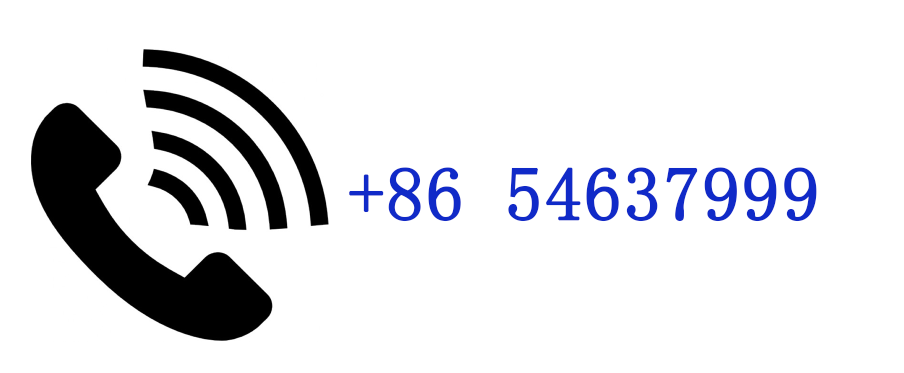
\includegraphics[height=2cm,width=7cm]{figures/Bushubtele.png}
\end{figure}



\newpage
	\bibliographystyle{IEEEtran}
	\bibliography{newrefs}
	
	
	
	
	
	
\begin{appendices}


\end{appendices}
\end{document}


